\chapter{Riemannian metrics (a quick tour)}

\begin{definition*}
    Let \(V\) be a (finite dimensional, \(\R\)-) vector space. An \dhighlight{inner product} is a 
    bilinear map
    \[g\in \Sigma^2 V^\star:V\times V\to \R\]
    which is 
    \begin{enumerate}
        \item[(i)] \dhighlight{symmetric} 
        \item[(ii)] \dhighlight{positive definite}: \(g(v,v)\geq 0, =0\iff v=0\) 
    \end{enumerate}
    We say that \((V,g)\) is an \dhighlight{inner product space}.
\end{definition*}

\begin{definition*}
    Let \(M\) be a manifold. A \dhighlight{Riemannian metric} \(g\in \Gamma(\Sigma^2 T^\star M)\)
    such that for all \(p\in M, (T_pM,g_p(\cdot,\cdot))\) is an inner product space. A pair \((M,g)\)
    is called a \dhighlight{Riemannian manifold}.
\end{definition*}

Note \(g_p\in (\Sigma^2T^\star M)_p=\Sigma^2(T_p M^\vee)\). \marginnote{This is just notation I use, because everyone does (talking about the postion of the p, after the \(T\)!)}

\begin{remark}
    If \(E\to M\) is an vector bundle, a metric on \(E\) is a section \(g\in \Gamma(\Sigma^2 E^\vee)\)
    s.t. \((E_p,g_p(\cdot,\cdot))\) is an inner product space.
\end{remark}

Note that on \(\R^n\) we have a frame \(\{dx_1,\dots,dx_n\}\) for \(T^\star \R^n\). More 
generally, \(T^2 T^\star \R^n\) admits a global frame \(\{dx_i\otimes dx_j\}_{1\leq i,j\leq n}\).
Hence, any section \(\sigma\in \Gamma(T^2 T^\star \R^n)\) can be written as 
\[\sigma=\sum_{i,j=1}^n\sigma_{ij}dx_i\otimes dx_j\]
for \(\sigma_{ij}:\R^n\to\R\).

Then \(\sigma\) is a metric iff:
\begin{enumerate}
    \item[(i)] \(\sigma_{ij}=\sigma_{ji}\), i.e. any symmetric matrix 
    \item[(ii)] \(\sum_{i,j=1^n}\sigma_{ij}v^i v^j\geq 0, =0\iff v=0 \)  
\end{enumerate}

in other words \(\sigma\in \Gamma(T^2 T^\star\R^n)\) defines a metric, iff
\((\sigma_{ij}):\R^n\to \text{Mat}(n\times n)\)
lands in the subspace of symmetric and positive definite matrices.

\begin{example}
    \(g_0\coloneqq \sum{i=1^n}dx_i\otimes dx_i=\sum_{i,j=1}^n \delta_{ij} dx_i\otimes dx_j\). We call 
    \(g_0\) the \dhighlight{Euclidean metric}.
\end{example}

\begin{definition*}
    Let \((M,g)\) be a Riemannian manifold.
    \begin{enumerate}
        \item[(1)] Given \(v\in T_pM\), the \dhighlight{length of \(v\)} \[|v|_g=\sqrt{g_p(v,v)}\]
        \item[(2)] Given \(v,w\in T_pM,v,w\neq 0\) the \dhighlight{angle between \(v,w\)} is the unique \(\theta\in [0,\pi]\)
                    \[\cos\theta = \frac{g_p(v,w)}{|v|_g|w|_g}\]
        \item[(3)] We say that \(v,w\in T_pM\) are orthogonal if \(g(v,w)=0\). 
    \end{enumerate} 
\end{definition*}

\dhighlight{Exercise:} If \(M=\R^n,g=g_0\) the above definitions recovers the classical definitions.

\begin{definition*}
    Given \(\gamma:[a,b]\to M\), the \dhighlight{length} of \(\gamma\) is given by 
    \[L_g(\gamma)\int_a^b|\underbrace{\dot{\gamma(t)}}_{\in T_{\gamma(t)}M}|dt\] 
    Given \(p,q\in M\), we define 
    \[d(p,q)=\inf \{L_g(\gamma)\mid \gamma:[a,b]\to M,  p=\gamma(a),q=\gamma(b)\}.\]
\end{definition*}

\begin{lemma}\label{lem:9.1}
    \(L_g(\gamma)\) does not depend on the parametrization. In other words if \(\gamma:[c,d]\to [a,b],\gamma'>0\)
    Then setting \(\sigma\coloneq \gamma\circ \phi\). We have 
    \[L_g(\sigma)=L_g(\gamma)\] 
\end{lemma}

\begin{proof}
    \begin{align*}
        L_g(\sigma)&=\int_c^d|\dot{\sigma}(t)|dt=\int_c^d|\dot{\gamma}(\sigma(\phi(t)))\dot{\phi}(t)|dt\\
        &=\int_c^d |\dot{\gamma}|\dot{\phi}(t)dt=\int_a^b|\dot{\gamma}(s)|ds=L_g(\gamma),
    \end{align*}
    where the last equality is just a change of variables.
\end{proof}

\dhighlight{Fact:} \((M,d_g(\cdot,\cdot))\) is a metric space.

The infimum in the definition can not be a minimum, take \(\R^2\setminus \{0\}\) with the euclidean metric, the distance is not different from the distance in \(\R\).

\begin{lemma}\label{lem:9.2}
    Let \(M\) be a smooth manifold. Then \(M\) admits a Riemannian 
    metric.
\end{lemma}

\begin{proof}
    Choose a covering of \(M\) \(\{U_\alpha\}_{\alpha\in \cA}\) by coordiante charts \(\varphi:U_\alpha\to \R^n\).
    Let \(\{\psi_\alpha\}_{\alpha\in \cA}\) be a partition of unity subject to the cover.
    Let \(g_\alpha=\varphi_\alpha^\star\in\Gamma(\Sigma^2 T^\star U_\alpha)\) and let \(g=\sum_{\alpha\in\cA}=\underbrace{\psi_\alpha g_\alpha}_{\in \Gamma(\Sigma^2T^\star M)}\).
    This makes sense by local finiteness. It is clear that \(g\) is a metric:

    It has to be symmetric, because the \(g_\alpha\) are symmetric. To check that \(g_p(v,v)> 0\)
    whenever \(v\neq 0\) note that \(\exists\alpha\) s.t. \(\psi_\alpha(p)>0\implies g_\alpha(v,v)>0\)
    whenever \(v\neq 0,\psi_\alpha g_\alpha(v,v)\geq 0\forall \alpha\)
\end{proof}

\begin{corollary}\label{lem:9.3}
    The space of Riemannian metrics on \(M\) is convex and non-empty, hence contractable.
\end{corollary}

\begin{proof}
    Exercise.
\end{proof}

\begin{lemma}\label{lem:9.4}
    Let \((W,g)\) be an inner product space. If \(V\stackrel{i}{\hookrightarrow} W\), then 
    \(g\) restricts to an inner product on \(V\). We can write \(g\restrict{V}=i^\star g(\cdot,\cdot),i^\star g(v,w)=g(i(v),i(w))\).
\end{lemma}

\begin{proof}
    Straightforward check, therefore omitted.
\end{proof}

\begin{corollary}\label{cor:9.5}
    Let \(i:M\hookrightarrow N\) an immersion. If \(g\in \Gamma(\Sigma^2T^\star N)\) is a 
    Riemannian metric, then \(i^\star g\in \Gamma(\Sigma^2 T^\star M)\) is also a metric and we call 
    \(i^\star g\) the \dhighlight{induced metric}. 
\end{corollary}

\begin{proof}
    By definition, \(di:T_p^M\to T_{i(p)}N\) is injective. Now apply lemma \ref{lem:9.4}.
\end{proof}

\begin{example}
    Suppose that \(M\hookrightarrow \R^n\) embedded submanifold. Then \(i^\star g_0\) is a 
    metric on \(M\).
    \begin{figure}[H]\label{fig:9.1}
        \centering
        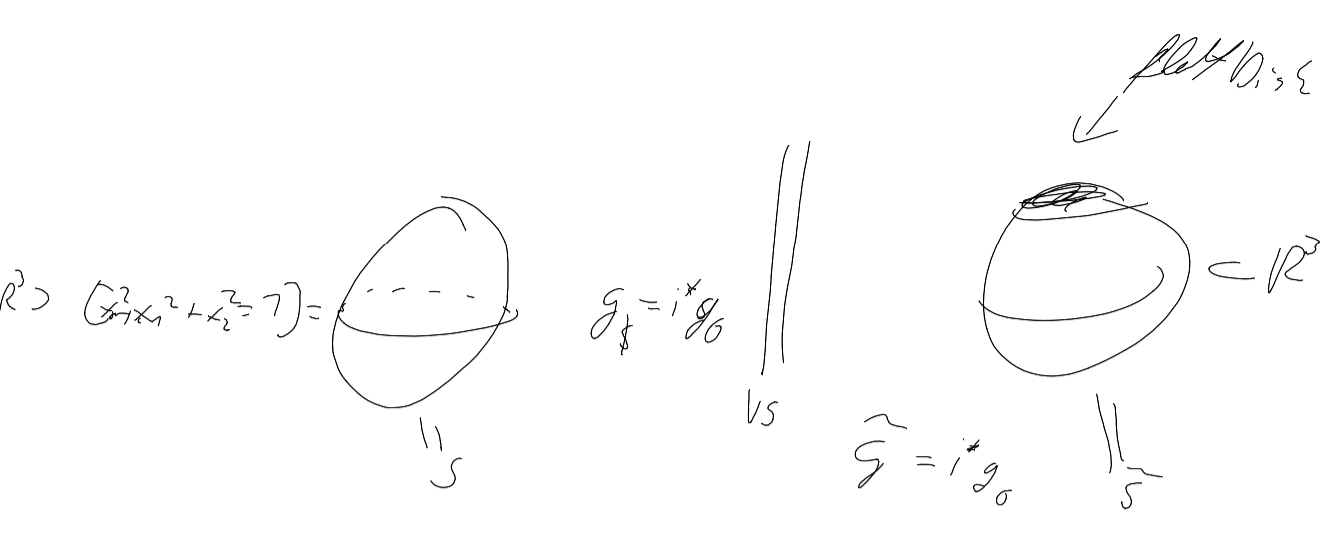
\includegraphics[width=.7\textwidth]{sketch_9_01.png}
        \caption{Sketch 9.1}
    \end{figure}
    He writes \(g_{\mathbb{S}}=i^\star g_0\). \marginnote{Everything after the fact that metrics exist is non-examable.}
    Question: does there exist a diffeomorphism \(\varphi:S\to \tilde{S}\) s.t. 
    \(\varphi^\star \tilde{g}=g_{\mathbb{S}}\)? The answer is no!

    Need: Invariant of Riemannian manifold.

\end{example}

Given \((M,g)\to R_g\in \Gamma(T^{3,1}TM)\) called the curvature tensor. We have 
\[\varphi^\star R_g=R_{\varphi^\star g},\]
for \(\varphi:M\to M'\) a diffeomorphism.

\dhighlight{Fact:} \(R_{g_0}\equiv 0\) and \(R_{g_{\mathbb{S}}}\iff \underbrace{s_{g}}_{\in C^\infty(S)}\equiv 1\).

Not only is there no global diffeomorphism, there is also no local diffeomorphism!


\markeol{21}
